\begin{slikaDesno}{fig/SH_kolo.pdf}
\PID Сигнал $x(t) = 2\sin\left( \upomega_0 t\right)$,
где је $\upomega_0 = 100\uppi$, доводи се на улаз кола са слике. Прекидач у колу је отворен, осим у 
тренуцима $t = kT$ када је \textit{краткотрајно} затворен ($k \in \mathbb Z$). 
Познато је $T = \dfrac{2\uppi}{\upomega_{\rm s}}$, $\upomega_{\rm s} = 800\uppi$.
Ако се излазни сигнал кола, $x_{\rm s}(t)$ 
обради идеалним филтром функције преноса $H(\jj\upomega) = 
a \rect\left(\dfrac{\upomega}{4\upomega_0} \right)$, 
израчунати константу $a$ тако да се као резулат добије тачно 
$y(t) = \sin\left( \upomega_0 t + \upphi \right)$, и том приликом израчунати угао $0 \leq \upphi < 2\uppi$.
\end{slikaDesno} \\


\textsc{\underline{Решење}}: Операциони појачавачи у колу повезани су у конфигурацију два јединична 
бафера. Сигнал на излазу левог операционог појачавача једнак је сигналу $x(t)$, 
док је напон на кондензатору једнак напону на излазу кола $x_{\rm s}(t)$. Када је прекидач отворен, 
напон кондензатора се не мења, док при краткотрајном затварању у тренуцима $kT$, напон кондензатора 
прима вредност $x(kT)$. Ово доводи до степеничастог напона, израђеног од низа правоугаоних импулса.

\begin{figure}[hb!]
    \begin{subfigure}[t]{0.35\textwidth}
        \centering
        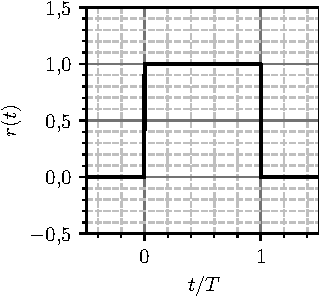
\includegraphics[scale=1]{fig/SH_plot_2.pdf}
        \caption{$r(t)$}        
        \label{fig:\ID.pulse}
    \end{subfigure}
    \hfill
    \begin{subfigure}[t]{0.55\textwidth}
        \centering
        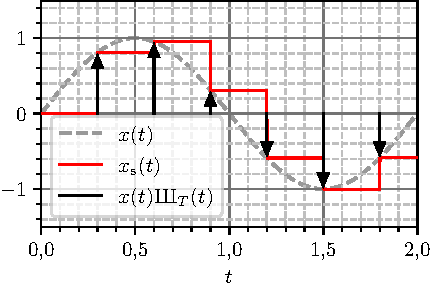
\includegraphics[scale=1]{fig/SH_plot_1.pdf}
        \caption{Уз пример, $T = 0,3$.}        
        \label{fig:\ID.primer}
    \end{subfigure}
    \caption{}
\end{figure}

Такав сигнал се може изградити помоћу низа померених правоугаоних јединичних импулса 
облика ${r(t) = \uu(t) - \uu(t - T)}$,
приказаних на слици \ref{fig:\ID.pulse}. Облик излазног сигнала се онда може представити као 
$x_{\rm s}(t) = \sum_{k = -\infty}^{\infty} x(kT) \cdot r(t - kT)$. Пошто се онда
конволуција са Дираковим импулсом може користити за померање у времену, односно важи
$r(t - kT) = r(t) \ast \updelta(t - kT)$, добијени израз се може трансформисати 
поступком\footnote{Користи се правило еквиваленције 
$x(kT) \updelta(t - kT) = x(t) \updelta(t - kT)$. }
  
\begin{equation}
x_{\rm s}(t) = \sum_{k = -\infty}^{\infty} x(kT) \cdot r(t - kT)    
             = \sum_{k = -\infty}^{\infty} x(kT) \cdot r(t) \ast \updelta(t - kT) = 
             r(t) \ast x(t) \III_T(t).  
\end{equation}

Тако добијени израз даје основу за фреквенцијску анализу сигнала. Одређивањем спектра 
таквог сигнала, применом теорема о трансформацији конволуције и производа, налазимо резултат:

\begin{eqnarray}
    X_{\rm s}(\jj\upomega) = \mathcal{FT}\{ x_{\rm s}(t) \}
    = R(\jj\upomega) \cdot \dfrac{1}{\cancel{2\uppi}} 
    \left(X(\jj\upomega) \ast 
    \underbrace{\dfrac{\cancel{2\uppi}}{T}}_{\upomega_0} \III_{\upomega_s}(\upomega) \right)
    =
    \dfrac{1}{T}
    R(\jj\upomega) \sum_{k = -\infty}^{\infty} X(\jj(\upomega - k\upomega_s)) \nonumber \\
\end{eqnarray}

Излаз након филтрирања идеалним филтром је онда облика 
$X_{\rm s}^{\text{(f)}}(\jj\upomega) = 
X_{\rm s}(\jj\upomega)\cdot H(\jj\upomega) = \dfrac{1}{T} R(\jj\upomega)
\sum_{k = -\infty}^{\infty} X(\jj(\upomega - k\upomega_s)) 
\cdot a \rect\left(\dfrac{\upomega}{4\upomega_0} \right)$. Пошто је задовољена 
теорема одабирања ($\upomega_{\rm s} > 2\upomega_{0}$) не долази до преклапања спектралних реплика, 
па тако идеални филтар који одбацује све чланове ван опсега 
$\left(-\dfrac{\upomega_0}{2}, \dfrac{\upomega_0}{2}\right)$ задржава само централну 
спектралну реплику, за $k = 0$, тиме остаје резултат филтрирања
$X_{\rm s}^{\text{(f)}}(\jj\upomega) = 
X_{\rm s}(\jj\upomega)\cdot H(\jj\upomega)$, односно 
$
    X_{\rm s}(\jj\upomega) = \dfrac{a}{T} R(\jj\upomega)  X(\jj(\upomega)).
$
Практично, може се сматрати да се цео систем од улаза до излаза, у општијем случају 
под претпоставком задовољења теореме одабирања, може представити једном функцијом преноса 
облика 
\begin{equation}
    G(\jj\upomega) = \dfrac{X_{\rm s}^{\text{(f)}}}{X(\jj\upomega)} = \dfrac{a R(\jj\upomega)}{T}. \label{eq:\ID.general}
\end{equation}


Заменом резултата за спектар датог правоугаоног импулса из задатка \ref{ID:rect_pulse_spectrum}
и спектра простопериодичног сигнала налазимо конкретан резултат за функцију преноса 
${G(\jj\upomega) = a \cdot \dfrac{1 - \ee^{-\jj\upomega T} }{\jj\upomega T}}$. Одређивањем функције преноса на учестаности
побуде $\upomega = \upomega_0$ налазе се појачање амплитуде и фазни померај излазног сигнала.  
\begin{align}
    |G(\jj\upomega_0)| = &\ a \left| \dfrac{1 - \ee^{-\jj\upomega T} }{\jj\upomega T} \right| = 
    \dfrac{ a\sqrt{2\bigl(1 - \cos(\upomega_0 T)\bigr)} }{\upomega_0 T} \\
    \arg G(\jj\upomega_0) = & \dfrac{\upomega_0 T - \uppi}{2} 
\end{align}
Пошто је према услову задатка $\upomega_0 T = \dfrac{\uppi}{4}$ коначно се добија да је 
$|G(\jj\upomega_0)| = \dfrac{4a}{\uppi} \sqrt{2 - \sqrt {2}}$ и $\upphi = -\dfrac{3\uppi}{8}$. Према услову задатка, 
амплитуда побудног и одзивног сигнала је иста, то мора бити $|G(\jj\upomega_0)| = 1$ па је 
$a = \dfrac{\uppi} { 4 \sqrt{2 - \sqrt {2}} }$.

Скренимо пажњу на општи закључак. Уколико је теорема одабирања задовољена, односно, уколико не долази до преклапања 
спектралних реплика, онда се резултат \ref{eq:\ID.general} може сматрати општим. Односно, он показује како облик 
реконструкционог импулса $r(t)$, утиче на спектар одзивног сигнала. 

Читаоцу се препоручује
да размотри какав се сигнал јавља на излазу целог система, уколико се уместо датог идеалног филтра 
пропусника ниских учестаности, $H(\jj\upomega)$ искористи филтар пропусник опсега учестаности, централне кружне учестаности $2 \upomega_0$. 
